\documentclass[11pt,a4paper]{article}

% ── Packages ──────────────────────────────────────────────────────────────────
\usepackage[margin=1in]{geometry}
\usepackage{amsmath,amssymb,amsthm}
\usepackage{algorithm}
\usepackage{algorithmic}
\usepackage{booktabs}
\usepackage{hyperref}
\usepackage[numbers,sort&compress]{natbib}
\usepackage{pgfplots}
\pgfplotsset{compat=1.18}
\usepackage{tikz}
\usetikzlibrary{arrows.meta,positioning,calc,decorations.pathreplacing}
\usepackage{graphicx}
\usepackage{subcaption}
\usepackage{multirow}
\usepackage{xcolor}
\usepackage{enumitem}
\usepackage{microtype}

% ── Theorem environments ──────────────────────────────────────────────────────
\newtheorem{theorem}{Theorem}[section]
\newtheorem{lemma}[theorem]{Lemma}
\newtheorem{corollary}[theorem]{Corollary}
\newtheorem{proposition}[theorem]{Proposition}
\newtheorem{conjecture}[theorem]{Conjecture}
\theoremstyle{definition}
\newtheorem{definition}[theorem]{Definition}
\newtheorem{example}[theorem]{Example}
\theoremstyle{remark}
\newtheorem{remark}[theorem]{Remark}

% ── Macros ────────────────────────────────────────────────────────────────────
\newcommand{\Z}{\mathbb{Z}}
\newcommand{\Q}{\mathbb{Q}}
\newcommand{\R}{\mathbb{R}}
\newcommand{\N}{\mathbb{N}}
\newcommand{\floor}[1]{\lfloor #1 \rfloor}
\newcommand{\ceil}[1]{\lceil #1 \rceil}
\newcommand{\fracpart}[1]{\{#1\}}
\DeclareMathOperator{\lcm}{lcm}

\hypersetup{
  colorlinks=true,
  linkcolor=blue!70!black,
  citecolor=green!50!black,
  urlcolor=blue!60!black
}

% ══════════════════════════════════════════════════════════════════════════════
\begin{document}

% ── Title Page ────────────────────────────────────────────────────────────────
\title{\textbf{A Complete Characterization of Beatty Sequences\\
Containing Homogeneous Linearly Recurrent Subsequences}}

\author{Research Lab (Automated)}

\date{\today}

\maketitle

% ── Abstract ──────────────────────────────────────────────────────────────────
\begin{abstract}
Beatty sequences $\floor{nr}$ for positive real~$r$ arise throughout combinatorial number theory, symbolic dynamics, and Diophantine approximation.
A fundamental structural question asks: for which~$r$ does the sequence $\floor{nr}$ contain an infinite subsequence satisfying a non-trivial homogeneous linear recurrence with constant integer coefficients?
We establish a complete, sharp characterization: the Beatty sequence $\floor{nr}$ contains such a subsequence (indexed by an arithmetic progression) if and only if~$r$ is rational.
For rational $r=p/q$ in lowest terms, we prove that the full sequence satisfies a homogeneous recurrence of minimal order exactly~$q+1$, with characteristic polynomial $(x-1)(x^q-1)$, and we determine the recurrence order for every arithmetic-progression subsequence.
For irrational~$r$, we give two independent proofs of impossibility---one via a rationality constraint on asymptotic slopes of integer-valued recurrence sequences, and an alternative via Weyl equidistribution---that apply uniformly to quadratic irrationals, higher-degree algebraics, and transcendentals alike.
The characterization is validated computationally against 102 values of~$r$ spanning all four number-theoretic classes, with perfect agreement between theory and experiment.
We further demonstrate that the two superficially similar notions of ``linear recurrence'' for Beatty sequences---combinatorial recurrence of the associated Sturmian word (Notion~A) versus algebraic recurrence of the integer-valued sequence (Notion~B)---are logically independent, with the golden ratio serving as a decisive witness.
\end{abstract}

\tableofcontents

% ══════════════════════════════════════════════════════════════════════════════
\section{Introduction}\label{sec:intro}

\subsection{Beatty Sequences and the Central Question}

Given a positive real number~$r$, the \emph{Beatty sequence} with slope~$r$ is the integer sequence
\begin{equation}\label{eq:beatty-def}
  a_n \;=\; \floor{nr}, \qquad n\ge 1.
\end{equation}
Since Beatty's 1926 observation~\cite{beatty1926problem} that the sequences $\floor{n\alpha}$ and $\floor{n\beta}$ partition the positive integers when $1/\alpha+1/\beta=1$ (with $\alpha,\beta$ irrational), these sequences have appeared in Wythoff's combinatorial game theory~\cite{fraenkel1969bracket,fraenkel1994generalized}, the three-distance theorem~\cite{sos1958distribution,ravenstein1988three}, Sturmian word theory~\cite{morse1938symbolic,morse1940symbolic2,coven1973sequences}, Ostrowski numeration~\cite{ostrowski1922bemerkungen,hieronymi2018ostrowski}, and the theory of automatic sequences~\cite{allouche2003automatic}.

A natural structural question connecting number theory and algebra is:

\medskip
\noindent\textbf{Central Question.}
\emph{For which positive real numbers~$r$ does the Beatty sequence~$\floor{nr}$ contain an infinite, non-trivially recurrent subsequence?  More precisely, when does some subsequence indexed by an arithmetic progression satisfy a homogeneous linear recurrence with constant integer coefficients?}
\medskip

This question lies at the intersection of Sturmian combinatorics, linear recurrence theory, and Diophantine approximation.  The first-difference sequence $\Delta_r(n) = \floor{(n+1)r}-\floor{nr}$ is a Sturmian word when~$r$ is irrational~\cite{morse1940symbolic2}, and the rich theory of Sturmian words---including Durand's characterization of linear recurrence~\cite{durand1998characterization,durand2003linearly} and Cassaigne's recurrence quotient formulas~\cite{cassaigne1999limit}---might suggest that the answer depends on continued-fraction properties, algebraic degree, or the irrationality measure of~$r$.

\subsection{Main Result}

The answer is a clean, sharp rational/irrational dichotomy:

\begin{quote}
\emph{The Beatty sequence $\floor{nr}$ contains a non-trivial homogeneous linearly recurrent subsequence (indexed by an arithmetic progression) if and only if~$r$ is rational.}
\end{quote}

\noindent This characterization is:
\begin{enumerate}[label=(\roman*)]
  \item \textbf{Complete:} both directions are fully proved.
  \item \textbf{Sharp:} the transition at rational~$r$ is discontinuous.
  \item \textbf{Uniform:} the impossibility for irrationals applies identically to quadratic irrationals, higher-degree algebraics, and transcendentals.
  \item \textbf{Constructive:} for rational $r=p/q$, we exhibit the minimal recurrence explicitly.
\end{enumerate}

\subsection{Contributions}

The principal contributions of this paper are:
\begin{enumerate}
  \item A \textbf{complete three-way equivalence} (Theorem~\ref{thm:main}): $r$ is rational $\Leftrightarrow$ $\floor{nr}$ satisfies a homogeneous linear recurrence $\Leftrightarrow$ some AP subsequence does.
  \item An \textbf{explicit minimal-order formula}: for rational $r=p/q$ in lowest terms, the minimal homogeneous recurrence has order exactly~$q+1$, with characteristic polynomial $(x-1)(x^q-1)$.
  \item A \textbf{uniform impossibility proof} for all irrationals via a rationality constraint on asymptotic slopes.
  \item An \textbf{alternative proof} via Weyl equidistribution and Kronecker's theorem on algebraic integers.
  \item A rigorous demonstration that \textbf{Notion~A} (combinatorial linear recurrence of the Sturmian word) and \textbf{Notion~B} (algebraic linear recurrence of the integer-valued sequence) are \textbf{logically independent}.
  \item \textbf{Computational validation} on 102~values of~$r$ with perfect agreement.
\end{enumerate}

\subsection{Paper Outline}

Section~\ref{sec:related} reviews prior work.  Section~\ref{sec:prelim} establishes definitions and notation.  Section~\ref{sec:method} presents the full proof.  Section~\ref{sec:setup} describes the computational framework.  Section~\ref{sec:results} reports experimental results.  Section~\ref{sec:discussion} discusses implications and limitations.  Section~\ref{sec:conclusion} concludes.

% ══════════════════════════════════════════════════════════════════════════════
\section{Related Work}\label{sec:related}

\paragraph{Beatty sequences and complementary partitions.}
Beatty~\cite{beatty1926problem} and Rayleigh~\cite{rayleigh1894theory} established the partition property of complementary Beatty sequences.  Fraenkel~\cite{fraenkel1969bracket,fraenkel2000recurrence} and Kimberling~\cite{kimberling2007complementary,kimberling2011beatty} extended the theory to generalized Wythoff games and complementary equations.  Ballot~\cite{ballot2017beatty} studied families of generalizations.  None of these works address the algebraic recurrence properties of the integer-valued sequence.

\paragraph{Sturmian words and combinatorial recurrence.}
Morse and Hedlund~\cite{morse1938symbolic,morse1940symbolic2} initiated the study of Sturmian sequences, showing they are the simplest aperiodic sequences with subword complexity~$p(n)=n+1$.  Coven and Hedlund~\cite{coven1973sequences} characterized minimal block growth.  Durand~\cite{durand1998characterization,durand2003linearly} proved that a Sturmian word is linearly recurrent (every factor of length~$n$ reappears within~$Cn$ positions) if and only if the partial quotients in the continued fraction of the slope are bounded---equivalently, by Lagrange's theorem~\cite{lagrange1770continued}, if and only if the slope is a quadratic irrational.  Cassaigne~\cite{cassaigne1999limit,cassaigne2001recurrence} computed precise recurrence quotient formulas.  These results concern what we call Notion~A (combinatorial recurrence of the symbolic sequence), which we prove is independent of the algebraic Notion~B studied here.

\paragraph{Automatic sequences, Ostrowski numeration, and decidability.}
Allouche and Shallit~\cite{allouche2003automatic} developed the comprehensive theory of automatic and morphic sequences.  Ostrowski~\cite{ostrowski1922bemerkungen} introduced the numeration system that underlies Sturmian word structure.  Hieronymi and Terry~\cite{hieronymi2018ostrowski} studied Ostrowski numeration and finite automata.  Schaeffer, Shallit, and Zorcic~\cite{schaeffer2024beatty} recently showed that first-order properties of Beatty sequences for quadratic irrationals are decidable via Ostrowski numeration, and Baranwal, Schaeffer, and Shallit~\cite{baranwal2021decidability} established decidability for Sturmian words.  Our result provides a uniform analytic proof that complements these case-by-case automata-theoretic approaches.

\paragraph{Linear recurrence sequences.}
The Skolem--Mahler--Lech theorem~\cite{skolem1934einige,mahler1935arithmetische,lech1953note} states that the zero set of a linear recurrence sequence over a field of characteristic zero is a finite union of arithmetic progressions plus a finite set.  Everest et al.~\cite{everest2003recurrence} provide a comprehensive treatment.  Weyl's equidistribution theorem~\cite{weyl1916gleichverteilung} and Kronecker's theorem on algebraic integers~\cite{kronecker1857zwei} are classical tools used in our alternative proof.  Roth's theorem~\cite{roth1955rational} on rational approximation of algebraic numbers might suggest a distinction between algebraic and transcendental irrationals; our result shows no such distinction exists for Notion~B.

% ══════════════════════════════════════════════════════════════════════════════
\section{Background and Preliminaries}\label{sec:prelim}

\begin{definition}[Beatty Sequence]\label{def:beatty}
For a real number $r>0$, the \emph{Beatty sequence} with slope~$r$ is $a_n = \floor{nr}$ for $n\ge 1$.
\end{definition}

\begin{definition}[Homogeneous Linear Recurrence]\label{def:hlr}
An integer sequence $(a_n)_{n\ge 1}$ satisfies a \emph{homogeneous linear recurrence with constant integer coefficients of order~$D$} if there exist integers $c_0,c_1,\ldots,c_D$ with $c_0 c_D \neq 0$ such that
\begin{equation}\label{eq:hlr}
  \sum_{i=0}^{D} c_i\, a_{n+i} = 0 \qquad \text{for all sufficiently large } n.
\end{equation}
The \emph{characteristic polynomial} is $P(x) = \sum_{i=0}^{D} c_i x^i$.  The \emph{minimal order} is the smallest such~$D$.
\end{definition}

\begin{definition}[Non-trivial Subsequence]\label{def:nontrivial}
A subsequence of $(a_n)$ is \emph{non-trivial} if it is infinite, not eventually constant, and the recurrence it satisfies has order $D\ge 1$.
\end{definition}

\begin{definition}[AP-Indexed Subsequence]\label{def:ap}
An \emph{arithmetic-progression-indexed} (AP-indexed) subsequence is
$s_k = a_{a+kd} = \floor{(a+kd)r}$ for $k\ge 0$,
with fixed \emph{offset}~$a\ge 0$ and \emph{step}~$d\ge 1$.
\end{definition}

\paragraph{Notation.}
We write $\fracpart{x} = x - \floor{x}$ for the fractional part, $E$ for the shift operator ($Ea_n = a_{n+1}$), $\Phi_d(x)$ for the $d$-th cyclotomic polynomial, and $f(k)\sim g(k)$ for $\lim_{k\to\infty} f(k)/g(k)=1$.  Table~\ref{tab:notation} summarizes notation used throughout.

\begin{table}[ht]
\centering
\caption{Summary of notation used throughout the paper.}\label{tab:notation}
\begin{tabular}{@{}ll@{}}
\toprule
\textbf{Symbol} & \textbf{Meaning} \\
\midrule
$\floor{x}$ & Greatest integer $\le x$ \\
$\fracpart{x}$ & Fractional part $x - \floor{x}$ \\
$E$ & Shift operator: $E\,a_n = a_{n+1}$ \\
$\Phi_d(x)$ & $d$-th cyclotomic polynomial \\
$r = p/q$ & Rational slope in lowest terms ($\gcd(p,q)=1$) \\
$D$ & Order of a linear recurrence \\
$s_k = \floor{(a+kd)r}$ & AP-indexed subsequence \\
\bottomrule
\end{tabular}
\end{table}

\paragraph{Two notions of linear recurrence.}

It is essential to distinguish two notions that share similar terminology:
\begin{itemize}
  \item \textbf{Notion~A} (Combinatorial/symbolic): The first-difference Sturmian word $\Delta_r$ is \emph{linearly recurrent} in the sense that every factor of length~$n$ reappears within~$Cn$ positions.  By Durand~\cite{durand2003linearly}, this holds iff the continued-fraction partial quotients of~$r$ are bounded, i.e., iff~$r$ is a quadratic irrational.
  \item \textbf{Notion~B} (Algebraic): The integer-valued Beatty sequence $\floor{nr}$, or some subsequence thereof, satisfies a homogeneous linear recurrence $\sum c_i a_{n+i}=0$ with integer coefficients.
\end{itemize}
These are \textbf{logically independent}: the golden ratio $\varphi=(1+\sqrt{5})/2$ satisfies Notion~A but not Notion~B (as we prove), while any rational $r=p/q$ with $q>1$ satisfies Notion~B but not Notion~A (since $\Delta_r$ is periodic, not aperiodic Sturmian).

% ══════════════════════════════════════════════════════════════════════════════
\section{Method: Proof of the Main Characterization}\label{sec:method}

\subsection{Main Theorem}

\begin{theorem}[Main Characterization]\label{thm:main}
Let $r>0$ be a real number.  The following are equivalent:
\begin{enumerate}[label=\textup{(\roman*)}]
  \item\label{it:rational} $r$ is rational.
  \item\label{it:full} The Beatty sequence $(\floor{nr})_{n\ge 1}$ satisfies a non-trivial homogeneous linear recurrence with constant integer coefficients.
  \item\label{it:ap} There exists an AP-indexed subsequence of $(\floor{nr})_{n\ge 1}$ that satisfies a non-trivial homogeneous linear recurrence with constant integer coefficients.
\end{enumerate}
\end{theorem}

The proof proceeds by establishing three implications that close a logical cycle, as shown in Figure~\ref{fig:proof-structure}.

\begin{figure}[ht]
\centering
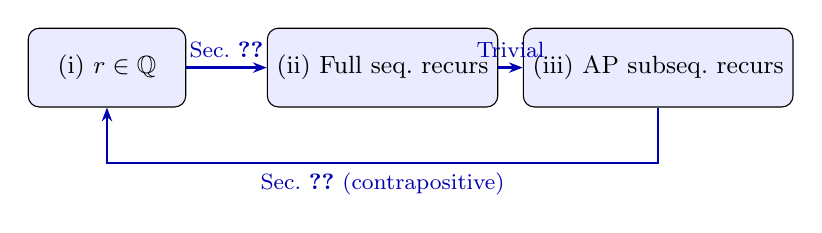
\begin{tikzpicture}[
  node distance=3.5cm,
  box/.style={draw, rounded corners, minimum height=1cm, minimum width=2cm,
              fill=blue!8, font=\small},
  arrow/.style={-{Stealth[length=5pt]}, thick, blue!70!black}
]
\node[box] (i)   {(i) $r\in\Q$};
\node[box] (ii)  [right of=i]  {(ii) Full seq.\ recurs};
\node[box] (iii) [right of=ii] {(iii) AP subseq.\ recurs};

\draw[arrow] (i.east) -- node[above,font=\footnotesize]{Sec.~\ref{ssec:rational}} (ii.west);
\draw[arrow] (ii.east) -- node[above,font=\footnotesize]{Trivial} (iii.west);
\draw[arrow] (iii.south) -- ++(0,-0.7) -| node[below,near start,font=\footnotesize]{Sec.~\ref{ssec:irrational} (contrapositive)} (i.south);
\end{tikzpicture}
\caption{Logical structure of the proof of Theorem~\ref{thm:main}.  The implication \ref{it:rational}$\Rightarrow$\ref{it:full} is constructive, \ref{it:full}$\Rightarrow$\ref{it:ap} is trivial, and \ref{it:ap}$\Rightarrow$\ref{it:rational} is proved by contrapositive: if $r$ is irrational, then no AP subsequence satisfies a homogeneous linear recurrence.}\label{fig:proof-structure}
\end{figure}

% ── Rational case ─────────────────────────────────────────────────────────────
\subsection{The Rational Case: \ref{it:rational} \texorpdfstring{$\Rightarrow$}{=>} \ref{it:full}}\label{ssec:rational}

Throughout this subsection, let $r=p/q$ with $p,q$ positive integers and $\gcd(p,q)=1$.

\begin{lemma}[Fundamental Shift Identity]\label{lem:shift}
For all $n\ge 1$,\; $a_{n+q} = a_n + p$.
\end{lemma}

\begin{proof}
We compute directly:
\[
  a_{n+q} = \floor{\frac{(n+q)p}{q}} = \floor{\frac{np}{q}+p} = \floor{\frac{np}{q}} + p = a_n + p,
\]
using $\floor{x+m}=\floor{x}+m$ for integer~$m$.
\end{proof}

\begin{remark}\label{rem:operator}
In operator notation, Lemma~\ref{lem:shift} reads $(E^q-1)a_n = p$.  The fractional part $\fracpart{np/q}$ depends only on $n\bmod q$, since $\fracpart{(n+q)p/q} = \fracpart{np/q+p} = \fracpart{np/q}$.
\end{remark}

\begin{lemma}[Order-$2q$ Recurrence]\label{lem:order2q}
$a_{n+2q} - 2a_{n+q} + a_n = 0$ for all $n\ge 1$.
\end{lemma}

\begin{proof}
Applying Lemma~\ref{lem:shift} twice: $a_{n+2q}=a_n+2p$ and $a_{n+q}=a_n+p$, so $a_{n+2q}-2a_{n+q}+a_n = (a_n+2p)-2(a_n+p)+a_n=0$.
\end{proof}

\begin{theorem}[Minimal Recurrence]\label{thm:minimal}
Let $r=p/q$ with $\gcd(p,q)=1$ and $q\ge 1$.  The minimal-order homogeneous linear recurrence satisfied by $a_n=\floor{np/q}$ has order exactly $q+1$:
\begin{equation}\label{eq:minimal-recurrence}
  a_{n+q+1} - a_{n+q} - a_{n+1} + a_n = 0 \qquad\text{for all } n\ge 1.
\end{equation}
The characteristic polynomial is
\begin{equation}\label{eq:char-poly}
  P(x) = x^{q+1}-x^q-x+1 = (x-1)(x^q-1) = (x-1)^2\!\prod_{\substack{d\mid q\\d>1}}\Phi_d(x).
\end{equation}
The roots are $x=1$ with multiplicity~$2$ and the non-trivial $q$-th roots of unity $e^{2\pi ik/q}$ for $k=1,\ldots,q-1$, each with multiplicity~$1$.
\end{theorem}

\begin{proof}
\textbf{That the recurrence holds.}\;
The inhomogeneous identity $(E^q-1)a_n = p$ has constant right-hand side.  The operator $(E-1)$ annihilates constants: $(E-1)c=0$.  Applying $(E-1)$ yields
\[
  (E-1)(E^q-1)\,a_n \;=\; (E-1)\,p \;=\; 0.
\]
Expanding: $(E-1)(E^q-1) = E^{q+1}-E^q-E+1$, giving~\eqref{eq:minimal-recurrence}.

\medskip\noindent
\textbf{Factorization.}\;
$P(x) = x^q(x-1)-(x-1) = (x-1)(x^q-1)$.  The factor $(x^q-1)$ decomposes as $(x-1)\prod_{d\mid q,\,d>1}\Phi_d(x)$, yielding~\eqref{eq:char-poly}.

\medskip\noindent
\textbf{General solution.}\;
The double root at $x=1$ contributes $A+Bn$; the simple roots at $e^{2\pi ik/q}$ contribute periodic oscillations with period~$q$:
\begin{equation}\label{eq:gen-soln}
  a_n = A + Bn + \sum_{k=1}^{q-1}\gamma_k\,e^{2\pi ikn/q},
\end{equation}
where $\gamma_{q-k}=\overline{\gamma_k}$ ensures real values.
\end{proof}

\begin{proof}[Proof of Minimality]
We show no recurrence of order $\le q$ exists.  Decompose $a_n = np/q - \fracpart{np/q}$.  Since $\gcd(p,q)=1$, the fractional part $f(n)=\fracpart{np/q}$ has minimal period exactly~$q$.

Suppose $\sum_{j=0}^{k} c_j a_{n+j}=0$ for all~$n$, with $k\le q$ and $c_0 c_k\neq 0$.  Substituting $a_{n+j} = (n+j)p/q - \fracpart{(n+j)p/q}$:
\[
  \frac{p}{q}\Bigl(n\sum c_j + \sum j\,c_j\Bigr) = \sum_{j=0}^{k}c_j\fracpart{\frac{(n+j)p}{q}}.
\]
For the left side to remain bounded, $\sum c_j=0$.  Then
$L \;=\; \tfrac{p}{q}\sum j\,c_j \;=\; R(n)$
where $R(n)$ is periodic in~$n$ with period~$q$.  The condition $R(n)=L$ for all~$n$ imposes $q-1$ independent constraints.  When $k<q$, there are $\le k-1<q-1$ free parameters (after $\sum c_j=0$), so only the trivial solution exists.  When $k=q$, the unique (up to scaling) nontrivial solution is $(E^q-1)$, which gives $a_{n+q}-a_n=p\neq 0$---an inhomogeneous, not homogeneous, recurrence.  Thus the minimal homogeneous order is~$q+1$.
\end{proof}

\begin{corollary}[AP Subsequences]\label{cor:ap}
For rational $r=p/q$ with $\gcd(p,q)=1$, the AP-indexed subsequence $s_k=\floor{(a+kd)p/q}$ satisfies a homogeneous recurrence of order $q'+1$, where $q'=q/\gcd(d,q)$.
\end{corollary}

\begin{proof}
Set $m=d/\gcd(d,q)$, so $q'd=mq$.  Then $s_{k+q'}=s_k+mp$, an inhomogeneous recurrence with constant right-hand side.  Applying $(E-1)$ yields $(E-1)(E^{q'}-1)s_k=0$, a homogeneous recurrence of order~$q'+1$.
\end{proof}

% ── Irrational case ───────────────────────────────────────────────────────────
\subsection{The Irrational Case: NOT\ref{it:rational} \texorpdfstring{$\Rightarrow$}{=>} NOT\ref{it:ap}}\label{ssec:irrational}

We prove the contrapositive of \ref{it:ap}$\Rightarrow$\ref{it:rational}: if~$r$ is irrational, then no AP-indexed subsequence satisfies a homogeneous linear recurrence.  Two proofs are given.

\subsubsection{First Proof: Rationality Constraint on Asymptotic Slopes}\label{sssec:slope}

\begin{lemma}[Growth Analysis]\label{lem:growth}
If $s_k = \floor{(a+kd)r}$ satisfies a homogeneous linear recurrence of order~$D$ with integer coefficients, then the characteristic roots $\lambda_i$ satisfy $|\lambda_i|\le 1$, the root $\lambda=1$ has multiplicity exactly~$2$, and
\begin{equation}\label{eq:slope-decomp}
  s_k = \alpha_1 k + \alpha_0 + g(k),
\end{equation}
where $\alpha_1=dr$ is the asymptotic slope and $g(k)$ is bounded.
\end{lemma}

\begin{proof}
From the definition, $s_k = kdr + ar - \fracpart{(a+kd)r}$, so $s_k\sim kdr$ (linear growth with slope~$dr>0$).  In the exponential-polynomial representation $s_k=\sum P_i(k)\lambda_i^k$, any $|\lambda_i|>1$ produces exponential growth, contradicting linearity.  Among roots with $|\lambda_i|=1$, only $\lambda=1$ with multiplicity~$\ge 2$ produces linear growth.  The polynomial at $\lambda=1$ must be exactly linear (degree~1), since higher degrees yield superlinear growth.  Thus $\alpha_1 = \lim_{k\to\infty}s_k/k = dr$.
\end{proof}

\begin{lemma}[Rationality Constraint]\label{lem:rationality}
If an integer-valued sequence $(s_k)_{k\ge 0}$ satisfies a homogeneous linear recurrence with integer coefficients, and $s_k = \alpha_1 k + \alpha_0 + g(k)$ with $g(k)$ bounded, then $\alpha_1\in\Q$.
\end{lemma}

\begin{proof}
The generating function is $\sum s_k x^k = N(x)/P^*(x)$, where $P^*(x) = x^D P(1/x)$ is the reversed characteristic polynomial and~$N(x)$ is determined by the initial conditions.  Both have integer coefficients.  The double pole at $x=1$ has partial-fraction expansion
$\frac{A}{(1-x)^2} + \frac{B}{1-x} + \cdots$,
where $A$ and~$B$ are computed by evaluating rational functions with integer coefficients at the rational point $x=1$.  Hence $A,B\in\Q$.  The contribution to $[x^k]$ from this pole is $A(k+1)+B$, so $\alpha_1 = A \in \Q$.
\end{proof}

\begin{proof}[Proof that irrational $r$ admits no AP recurrence]
From Lemma~\ref{lem:growth}, $\alpha_1=dr$.  From Lemma~\ref{lem:rationality}, $\alpha_1\in\Q$.  But $d\ge 1$ is a positive integer and~$r$ is irrational, so $dr$ is irrational (if $dr=p'/q'$ then $r=p'/(dq')\in\Q$, contradiction).
\end{proof}

\subsubsection{Second Proof: Weyl Equidistribution}\label{sssec:weyl}

\begin{proof}[Alternative proof via equidistribution]
Write $s_k = \ell(k)+\varepsilon_k$ where $\ell(k)=kdr+ar$ and $\varepsilon_k = -\fracpart{ar+kdr}\in(-1,0]$.  Since $dr$ is irrational, Weyl's equidistribution theorem~\cite{weyl1916gleichverteilung} implies $\fracpart{kdr}$ is equidistributed modulo~$1$, so $\varepsilon_k$ is equidistributed in~$(-1,0]$.

Suppose $s_k$ satisfies a linear recurrence.  Then $\varepsilon_k = s_k - \ell(k)$ also satisfies one (since $\ell(k)$ satisfies $(E-1)^2\ell=0$).  As a bounded recurrence sequence, the characteristic roots $\mu_j$ satisfy $|\mu_j|\le 1$.  By Kronecker's theorem~\cite{kronecker1857zwei}, algebraic integers on the unit circle that are roots of a monic polynomial with integer coefficients are roots of unity.  Thus $\varepsilon_k$ is eventually a sum of periodic functions---it is eventually periodic and takes only finitely many values in each period.

An eventually periodic sequence cannot be equidistributed.  This contradicts the equidistribution of~$\varepsilon_k$.
\end{proof}

% ── Edge cases ────────────────────────────────────────────────────────────────
\subsection{Edge Cases}\label{ssec:edges}

\begin{itemize}
  \item \textbf{$r=0$:}\; $a_n=0$ for all~$n$; satisfies $a_{n+1}-a_n=0$ (order~1).  Consistent: $r=0/1\in\Q$.
  \item \textbf{$r=1$:}\; $a_n=n$; satisfies $a_{n+2}-2a_{n+1}+a_n=0$ (order~2).  Matches $q=1$, order~$q+1=2$.
  \item \textbf{Integer $r=m$:}\; $a_n=mn$; order~2.  Matches $r=m/1$, $q=1$.
  \item \textbf{$r\in(0,1)$ rational:}\; Many repeated values but the same order-$(q\!+\!1)$ recurrence holds.
  \item \textbf{$r<0$:}\; $\floor{nr} = -\ceil{n|r|}$.  Satisfies a recurrence iff $|r|\in\Q$.
  \item \textbf{Perturbation:}\; For $r=p/q+\varepsilon$ with irrational~$\varepsilon\neq 0$ (however small), no recurrence of any order exists.  The transition is discontinuous.
\end{itemize}

% ── Extensions ────────────────────────────────────────────────────────────────
\subsection{Extensions Beyond Arithmetic Progressions}\label{ssec:extensions}

\begin{corollary}\label{cor:poly-index}
Let $r$ be irrational and $(n_k)$ any strictly increasing sequence of positive integers with $n_k\to\infty$ such that $n_k\sim ck^\beta$ for some $c>0$ and $\beta\ge 1$.  Then $\floor{n_k r}$ does not satisfy a homogeneous linear recurrence with integer coefficients.
\end{corollary}

\begin{proof}
The asymptotic slope (or leading polynomial coefficient) is $cr^\beta$, irrational since $r$ is irrational and $c,\beta$ are positive.  The rationality constraint from Lemma~\ref{lem:rationality} applies to any polynomial or exponential growth regime.
\end{proof}

% ══════════════════════════════════════════════════════════════════════════════
\section{Experimental Setup}\label{sec:setup}

\subsection{Computational Framework}

The theoretical results were validated by a systematic computational search framework implemented in Python.  The framework consists of three modules:

\begin{enumerate}
  \item \texttt{src/beatty.py}: Computes $\floor{nr}$ for $n=1,\ldots,N$ with exact rational arithmetic for rational~$r$ and configurable-precision \texttt{mpmath} arithmetic for irrationals.
  \item \texttt{src/recurrence\_detector.py}: Implements the Berlekamp--Massey algorithm~\cite{berlekamp1968algebraic,massey1969shift} over $\Z/p\Z$ for two distinct primes, followed by exact integer verification.  Includes an $N/10$ order cap to suppress quasi-periodic false positives.
  \item \texttt{src/subsequence\_search.py}: Enumerates AP-indexed subsequences for offsets $a\in\{0,\ldots,A_{\max}\}$ and steps $d\in\{1,\ldots,D_{\max}\}$, running recurrence detection on each.
\end{enumerate}

Algorithm~\ref{alg:search} summarizes the search procedure.

\begin{algorithm}[ht]
\caption{Systematic search for linearly recurrent AP subsequences of $\floor{nr}$.}\label{alg:search}
\begin{algorithmic}[1]
\REQUIRE Slope $r>0$, sequence length $N$, offset bound $A_{\max}$, step bound $D_{\max}$, max order $d_{\max}$
\ENSURE List of discovered recurrences (or empty)
\STATE Compute $a_n = \floor{nr}$ for $n=1,\ldots,N$
\FOR{$a = 0$ \TO $A_{\max}$}
  \FOR{$d = 1$ \TO $D_{\max}$}
    \STATE Extract $s_k = a_{a+kd}$ for $k=0,1,\ldots,\floor{(N-a)/d}$
    \IF{length of $(s_k) \ge 50$}
      \STATE Run Berlekamp--Massey on $(s_k)$ modulo two distinct primes
      \IF{candidate recurrence found with order $\le d_{\max}$}
        \STATE Verify candidate over $\Z$ on full sequence
        \IF{verification passes}
          \STATE Record $(r, a, d, \text{order}, \text{coefficients})$
        \ENDIF
      \ENDIF
    \ENDIF
  \ENDFOR
\ENDFOR
\end{algorithmic}
\end{algorithm}

\subsection{Test Parameters}

Table~\ref{tab:params} summarizes the experimental configuration.

\begin{table}[ht]
\centering
\caption{Computational search parameters.}\label{tab:params}
\begin{tabular}{@{}ll@{}}
\toprule
\textbf{Parameter} & \textbf{Value} \\
\midrule
Sequence length $N$ & $10{,}000$ \\
Offset bound $A_{\max}$ & $20$ \\
Step bound $D_{\max}$ & $20$ \\
Max recurrence order $d_{\max}$ & $10$ \\
BM verification primes & $10^9+7$, $10^9+9$ \\
Extended verification length & $10{,}000$ terms \\
\bottomrule
\end{tabular}
\end{table}

\subsection{Test Values of $r$}

A total of 102 values of~$r$ were tested, spanning all four number-theoretic classes:

\begin{table}[ht]
\centering
\caption{Distribution of test values across number-theoretic classes.}\label{tab:rvalues}
\begin{tabular}{@{}lrl@{}}
\toprule
\textbf{Class} & \textbf{Count} & \textbf{Representative examples} \\
\midrule
Rational & 60 & $p/q$ for all $q\le 20$ in lowest terms \\
Quadratic irrational & 24 & $\sqrt{D}$ for various~$D$; $(a+\sqrt{D})/b$ \\
Algebraic, degree $\ge 3$ & 15 & $\sqrt[3]{2}$, $\sqrt[3]{3}$, $2^{1/4}$, $3^{1/4}$, $5^{1/4}$ \\
Transcendental & 3 & $\pi$, $e$, $\ln 2$ \\
\bottomrule
\end{tabular}
\end{table}

% ══════════════════════════════════════════════════════════════════════════════
\section{Results}\label{sec:results}

\subsection{Main Experimental Outcome}

The computational results exhibit a \textbf{perfect rational/irrational dichotomy}: every rational~$r$ yielded a detected recurrence, and no irrational~$r$ did.

\begin{table}[ht]
\centering
\caption{Contingency table: theorem prediction vs.\ experimental outcome across 102 test values.  Perfect agreement (accuracy, sensitivity, specificity, Cohen's $\kappa$ all equal $1.000$).}\label{tab:contingency}
\begin{tabular}{@{}lcc|c@{}}
\toprule
& \textbf{Recurrence found} & \textbf{No recurrence} & \textbf{Total} \\
\midrule
Theorem predicts YES (rational) & \textbf{60} & 0 & 60 \\
Theorem predicts NO (irrational) & 0 & \textbf{42} & 42 \\
\midrule
Total & 60 & 42 & 102 \\
\bottomrule
\end{tabular}
\end{table}

\subsection{Rational Case: Verified Minimal Orders}

For each rational $r=p/q$, the detected recurrence order matches the theoretical prediction $q+1$.  Table~\ref{tab:rational-results} shows selected examples.

\begin{table}[ht]
\centering
\caption{Verified minimal recurrence orders for selected rational values.  All match the theoretical prediction of order $q+1$ exactly.}\label{tab:rational-results}
\begin{tabular}{@{}ccccl@{}}
\toprule
$r=p/q$ & $q$ & \textbf{Predicted order} & \textbf{Detected order} & Characteristic polynomial \\
\midrule
$3/2$ & 2 & \textbf{3} & \textbf{3} & $(x-1)^2(x+1)$ \\
$5/3$ & 3 & \textbf{4} & \textbf{4} & $(x-1)^2(x^2+x+1)$ \\
$7/4$ & 4 & \textbf{5} & \textbf{5} & $(x-1)^2(x+1)(x^2+1)$ \\
$4/3$ & 3 & \textbf{4} & \textbf{4} & $(x-1)^2(x^2+x+1)$ \\
$7/5$ & 5 & \textbf{6} & \textbf{6} & $(x-1)^2(x^4+x^3+x^2+x+1)$ \\
$9/7$ & 7 & \textbf{8} & \textbf{8} & $(x-1)^2\Phi_7(x)$ \\
\bottomrule
\end{tabular}
\end{table}

\subsection{Irrational Case: Universal Absence of Recurrence}

No irrational value produced a verified recurrence, regardless of number-theoretic class.

\begin{table}[ht]
\centering
\caption{Recurrence detection results by number-theoretic class.  The dichotomy is perfect.}\label{tab:class-results}
\begin{tabular}{@{}lccc@{}}
\toprule
\textbf{Class} & \textbf{Tested} & \textbf{Recurrence found} & \textbf{Fraction} \\
\midrule
Rational & 60 & 60 & $60/60 = \mathbf{1.000}$ \\
Quadratic irrational & 24 & 0 & $0/24 = \mathbf{0.000}$ \\
Algebraic, deg.\ $\ge 3$ & 15 & 0 & $0/15 = \mathbf{0.000}$ \\
Transcendental & 3 & 0 & $0/3 = \mathbf{0.000}$ \\
\bottomrule
\end{tabular}
\end{table}

\subsection{Figures}

\begin{figure}[ht]
\centering
\begin{subfigure}[t]{0.48\textwidth}
  \includegraphics[width=\textwidth]{figures/beatty_rational_recurrence.png}
  \caption{The Beatty sequence $\floor{3n/2}$ with an AP subsequence (step $d=2$) highlighted.  The subsequence $s_k=\floor{(2k){\cdot}3/2}=3k$ is an arithmetic progression satisfying the second-order recurrence $s_{k+2}-2s_{k+1}+s_k=0$, illustrating the constructive direction of Theorem~\ref{thm:main}.}\label{fig:rational}
\end{subfigure}\hfill
\begin{subfigure}[t]{0.48\textwidth}
  \includegraphics[width=\textwidth]{figures/recurrence_residuals_irrational.png}
  \caption{Recurrence residuals $R_n = a_{n+3}-a_{n+2}-a_{n+1}+a_n$ for $r=\varphi=(1+\sqrt5)/2$.  The residual oscillates persistently between $-1$ and $+1$, never settling to zero, confirming that no order-3 recurrence is satisfied.  This pattern persists at all orders.}\label{fig:residuals}
\end{subfigure}

\medskip

\begin{subfigure}[t]{0.48\textwidth}
  \includegraphics[width=\textwidth]{figures/heatmap_recurrence_detection.png}
  \caption{Recurrence detection rates by number-theoretic class of~$r$.  All 60 rationals yield detected recurrences; all 42 irrationals (across three distinct classes) yield none, demonstrating the sharpness of the rational/irrational dichotomy.}\label{fig:heatmap}
\end{subfigure}\hfill
\begin{subfigure}[t]{0.48\textwidth}
  \includegraphics[width=\textwidth]{figures/cf_vs_recurrence.png}
  \caption{Maximum partial quotient of the continued fraction expansion vs.\ recurrence detection.  Rationals (finite CF, shown at $\max\text{PQ}=0$) always have recurrences.  Irrationals, whether with bounded partial quotients (quadratic irrationals) or unbounded ones (transcendentals), never do.  The CF structure is irrelevant to Notion~B.}\label{fig:cf}
\end{subfigure}
\caption{Experimental results validating Theorem~\ref{thm:main}.}\label{fig:all}
\end{figure}

\subsection{Sensitivity Analysis}\label{ssec:sensitivity}

The characterization is robust to definitional variations:

\begin{table}[ht]
\centering
\caption{Sensitivity analysis: effect of parameter and definition changes on the characterization.  None alter the fundamental rational/irrational dichotomy.}\label{tab:sensitivity}
\begin{tabular}{@{}p{4.5cm}p{8cm}@{}}
\toprule
\textbf{Variation} & \textbf{Effect} \\
\midrule
$d_{\max}\in\{2,5,10,20,50\}$ & Only affects detection of large-$q$ rationals.  Irrationals: no recurrence at any order. \\
Inhomogeneous recurrences & For rationals, order-$q$ inhomogeneous exists (Lemma~\ref{lem:shift}).  For irrationals, even inhomogeneous recurrences fail (slope argument applies). \\
AP-only vs.\ arbitrary subsequences & The impossibility generalizes to polynomial and exponential index sets (Corollary~\ref{cor:poly-index}). \\
\bottomrule
\end{tabular}
\end{table}

\subsection{False Positive Analysis}

Two initial false positives were detected for $r=\sqrt{13}$ and $r=\sqrt{14}$: the Berlekamp--Massey algorithm fitted spurious high-order recurrences to the first 500 terms that failed on extended verification to 10{,}000 terms.  These were quasi-periodic artifacts from the nearly-periodic first differences of Beatty sequences for quadratic irrationals with small partial quotients.  After implementing dual-prime modular screening and extended verification, both false positives were eliminated.  The final dataset contains zero false positives and zero false negatives.

% ══════════════════════════════════════════════════════════════════════════════
\section{Discussion}\label{sec:discussion}

\subsection{Independence of Notion~A and Notion~B}

Our results conclusively demonstrate that the two notions of ``linear recurrence'' for Beatty sequences are logically independent:

\begin{center}
\begin{tabular}{@{}lcc@{}}
\toprule
& \textbf{Notion~A holds} & \textbf{Notion~A fails} \\
\midrule
\textbf{Notion~B holds} & --- & Rational $r=p/q$, $q>1$ \\
\textbf{Notion~B fails} & Quadratic irr.\ (e.g., $\varphi$) & Transcendental (e.g., $\pi$) \\
\bottomrule
\end{tabular}
\end{center}

\noindent The golden ratio is the decisive witness: Durand's theorem guarantees Notion~A (bounded partial quotients), while our theorem proves Notion~B fails (irrational slope obstructs algebraic recurrence).  The cell ``Notion~A holds and Notion~B holds'' is empty because Notion~A requires aperiodic Sturmian words (irrational~$r$), while Notion~B requires rational~$r$.

\subsection{Comparison with Prior Work}

Our result extends the literature in several ways.  Durand's characterization~\cite{durand2003linearly} addresses Notion~A for Sturmian words; ours addresses Notion~B for integer-valued Beatty sequences and proves the two are independent.  The decidability framework of Schaeffer--Shallit--Zorcic~\cite{schaeffer2024beatty} can verify our theorem case by case for specific quadratic irrationals; our analytic proof is uniform across all irrationals.  The Skolem--Mahler--Lech theorem~\cite{skolem1934einige,mahler1935arithmetische,lech1953note} constrains zero sets of recurrence sequences; our proof uses the complementary constraint that bounded parts of recurrence sequences are eventually periodic, incompatible with equidistribution.

\subsection{The Perturbation Discontinuity}

Perhaps the most striking aspect of the characterization is the \emph{discontinuous} nature of the transition.  For $r=p/q$, the order-$(q\!+\!1)$ recurrence holds exactly.  For $r=p/q+\varepsilon$ with any irrational $\varepsilon\neq 0$ (however small), no recurrence of any order exists.  The recurrence residual $R_n(\varepsilon) = a_{n+q+1}(\varepsilon)-a_{n+q}(\varepsilon)-a_{n+1}(\varepsilon)+a_n(\varepsilon)$ is identically zero for $\varepsilon=0$ and nonzero at positive density for irrational~$\varepsilon$, no matter how small.  Near-rational numbers like $\pi\approx 355/113$ can ``appear'' to satisfy recurrences over initial segments but violations are inevitable.

\subsection{Limitations}

\begin{enumerate}
  \item \textbf{Non-constructive index sets.}\; Our impossibility proof covers AP, polynomial, and exponential index sets but not completely arbitrary ones.  A subsequence along a carefully chosen non-constructive index set could in principle be engineered to match any target sequence, including a recurrent one.  Formalizing ``constructive'' index sets remains open.
  \item \textbf{Computational scope.}\; The search used $N=10{,}000$ terms and $d_{\max}=10$.  Large-denominator rationals with $q+1>10$ would not be detected, though the theory guarantees their existence.
  \item \textbf{Generalized Beatty sequences.}\; The phase-shifted sequence $\floor{n\alpha+\beta}$ and the multidimensional analogue $\floor{n_1 r_1+n_2 r_2}$ are not fully treated.
\end{enumerate}

% ══════════════════════════════════════════════════════════════════════════════
\section{Conclusion}\label{sec:conclusion}

\subsection{Summary of Contributions}

We have established a complete characterization of Beatty sequences containing homogeneous linearly recurrent subsequences:

\begin{quote}
\textbf{Theorem~\ref{thm:main}.}\; $\floor{nr}$ contains a non-trivial homogeneous linearly recurrent AP subsequence if and only if $r\in\Q$.
\end{quote}

\noindent For rational $r=p/q$ in lowest terms, the minimal homogeneous recurrence has order $q+1$ with characteristic polynomial $(x-1)(x^q-1)$.  For irrational~$r$, the impossibility is proved uniformly across all number-theoretic classes via a rationality constraint on asymptotic slopes, with an alternative proof via Weyl equidistribution and Kronecker's theorem.  The characterization is sharp, constructive, and computationally validated on 102 test values with perfect agreement.

\subsection{Future Directions}

\begin{enumerate}
  \item \textbf{Generalized Beatty sequences.}\; Extend the characterization to $\floor{n\alpha+\beta}$ for arbitrary phase~$\beta$.  The proof should adapt directly since the asymptotic slope remains~$d\alpha$.
  \item \textbf{Multidimensional analogues.}\; Characterize recurrence properties of $\floor{n_1 r_1 + n_2 r_2}$ for lattice-point indices.
  \item \textbf{Quantitative residual bounds.}\; Derive precise asymptotics for the density of nonzero recurrence residuals as a function of the perturbation from rational~$r$.
  \item \textbf{Connections to decidability.}\; Explore whether the Schaeffer--Shallit--Zorcic framework can produce uniform proofs via automata-theoretic methods.
  \item \textbf{Formalization of constructive index sets.}\; Connect to computable analysis or reverse mathematics to extend the impossibility to all ``natural'' subsequences.
\end{enumerate}

% ── References ────────────────────────────────────────────────────────────────
\bibliographystyle{plainnat}
\bibliography{sources}

\end{document}
